\documentclass[12pt]{article}
\usepackage{lingmacros}
\usepackage{mathtools}
\usepackage{tree-dvips}

\usepackage{tikz}
\usetikzlibrary{positioning}

\begin{document}

\section*{DevSpaces}

Don't forget to include examples of topicalization.
They look like this:

{\small
\enumsentence{Topicalization from sentential subject:\\ 
\shortex{7}{a John$_i$ [a & kltukl & [el & 
  {\bf l-}oltoir & er & ngii$_i$ & a Mary]]}
{ & {\bf R-}clear & {\sc comp} & 
  {\bf IR}.{\sc 3s}-love   & P & him & }
{John, (it's) clear that Mary loves (him).}}
}


\section{DevSpaces for Education}
Since \LaTeX\ is a markup language, any text we
type appears on the page, unless it contains
one of the nine reserved characters of \LaTeX, listed
below.

\begin{equation}
dX_{t}=\mu (X_{t},t)\,dt+\sigma (X_{t},t)\,dW_{t}
\end{equation}

If we want those characters to appear on the page, we
must precede them by a backslash, or, in the special
case of the backslash itself, we must use the 
command \verb(\verb(.  In math mode, we can use the command
\verb(\backslash(.

Note that there are three kinds of dash-objects.  Hyphens 
are very short, and are typed the way you would expect, using
"-".  Dashes, as in the range 1--2, are wider, and are typed
using \verb+--+.  If you feel a need for a wide---dash, you can
use \verb+---+.

\textbf{Dynamic Recompile}

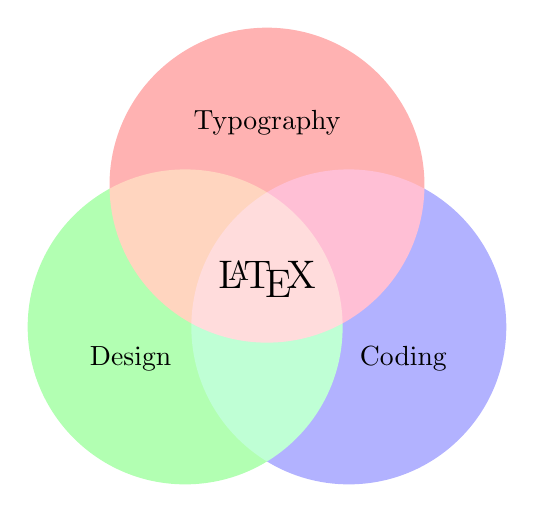
\begin{tikzpicture}
    \begin{scope}[blend group = soft light]
      \fill[red!30!white]   ( 90:1.2) circle (2);
      \fill[green!30!white] (210:1.2) circle (2);
      \fill[blue!30!white]  (330:1.2) circle (2);
    \end{scope}
    \node at ( 90:2)    {Typography};
    \node at ( 210:2)   {Design};
    \node at ( 330:2)   {Coding};
    \node [font=\Large] {\LaTeX};
  \end{tikzpicture}

\subsection{Diagram}
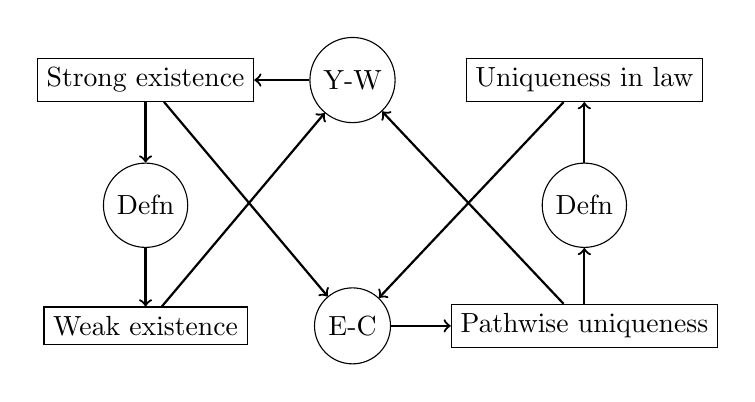
\begin{tikzpicture}
\matrix [column sep=7mm, row sep=5mm] {
  \node (se) [draw, shape=rectangle] {Strong existence}; &
  \node (yw) [draw, shape=circle] {Y-W}; &
  \node (ul) [draw, shape=rectangle] {Uniqueness in law}; \\
  \node (d1) [draw, shape=circle] {Defn}; & &
  \node (d2) [draw, shape=circle] {Defn}; \\
  \node (we) [draw, shape=rectangle] {Weak existence}; &
  \node (ec) [draw, shape=circle] {E-C}; &
  \node (pu) [draw, shape=rectangle] {Pathwise uniqueness}; \\
};
\draw[->, thick] (se) -- (d1);
\draw[->, thick] (d1) -- (we);
\draw[->, thick] (we) -- (yw);
\draw[->, thick] (yw) -- (se);
\draw[->, thick] (se) -- (ec);
\draw[->, thick] (ul) -- (ec);
\draw[->, thick] (ec) -- (pu);
\draw[->, thick] (pu) -- (yw);
\draw[->, thick] (pu) -- (d2);
\draw[->, thick] (d2) -- (ul);
\end{tikzpicture}

\section{Units}
Lengths in \LaTeX\ can be given in a number of Units.\\
\begin{tabular}{ll}
cm & Centimeters\\
em & The width of the letter M in the current font\\
ex & The height of the letter x in the current font\\
in & Inches\\
pc & Picas (1pc = 12pt)\\
pt & Points (1in = 72pt)\\
mm & Millimeters
\end{tabular}


Mood changes when there is a topic, as well as when
there is WH-movement.  \emph{Irrealis} is the mood when
there is a non-subject topic or WH-phrase in Comp.
\emph{Realis} is the mood when there is a subject topic
or WH-phrase.

\end{document}
